% Chapter 1

\chapter{Tube Including Mixing Vanes : DEBORA-Promoteur and AGATE-Promoteur Experiments} % Chapter title

\label{ch:debora_agate_prom} % For referencing the chapter elsewhere, use \autoref{ch:introduction} 

\section{Introduction}

In PWR cores, the industrial geometry is tremendously complex compared to traditional experimental setup usually consisting of simple tubes such as in the DEBORA experiment (Chapter \ref{chap:debora}). Although simple geometries are absolutely mandatory for verification and validation of the multi-physics modeling involved in boiling two-phase flows, it would hardly suffice to be extended to full scale industrial configurations. 

\npar

To that extent, there is a need for experimental measurements both in representative flow conditions \textbf{\underline{and}} geometry. This implies reproducing test sections including complicated shapes such as grids inducing significant transverse flow and turbulent mixing. 

\npar

In this Chapter, we describe the experimental setup called DEBORA-Promoteur and propose some analyses of former experimental measurements. Finally, its single-phase counterpart called AGATE-Promoteur is also presented.



\section{DEBORA-Promoteur}

\subsection{Test Section and Experimental Campaigns}

In 2003, the wish to investigate boiling flows in complex geometries similar to those of PWR fuel assembly motivated CEA and EDF to perform modifications of the DEBORA facility. In order to mimic the turbulent mixing induced by the grids holding the fuel rods, a mixing device equipped with blades was built with respect to the geometrical properties of the mixing vanes of the PWR grids (Figure \ref{fig:debprom_vanes}).


\begin{figure}[!h]
\centering
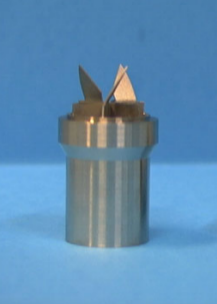
\includegraphics[width=0.2\linewidth]{img/DEBORA-Promoteur/prom_pic.png}
\caption{Picture of the mixing device.}
\label{fig:debprom_vanes}
\end{figure}

\npar

This mixing device was then welded into the DEBORA test section, thus named DEBORA-Promoteur. Its position upstream the end of the heating length was meant to induce a strong rotation in the flow in order to quantify the impact of the mixing regarding:

\begin{itemize}
\item Bubble recondensation for subcooled boiling ;
\item Void redistribution for saturated cases ;
\item Critical Heat Flux value compared to the naked pipe case.
\end{itemize}


The same measurement instrumentation as the DEBORA C3000 cases   (bi-optical probe, Figure \ref{fig:optical_probe}) was used to study the flow topology in the DEBORA-Promoteur experiment. In that regard, two measurements campaign were conducted:

\begin{itemize}
\item Campaign C4800 where the mixing vanes were placed $23.5\ D_{h}$ ($\approx 0.45$\ m)upstream the end of the heating length ;
\item Campaign C5200, where the mixing vanes were placed $10\ D_{h}$ ($\approx 0.19$\ m) upstream the end of the heating length.
\end{itemize}

\begin{note*}{}
Unfortunately, no thermal measurement campaign was conducted on the DEBORA-Promoteur facility.
\end{note*}

The different cases of the DEBORA-Promoteur experiment follow the same nomenclature as the DEBORA ones (Section \ref{sec:deb_exp_campaign}). A total of three test series were conducted:

\begin{enumerate}
\item Series 48G3P26W23 ;
\item Series 52G3P26W23 ; 
\item Series 52G3P26W27.
\end{enumerate}




\section{Boiling freon in a tube with mixing vanes : DEBORA-Promoteur experiments}
\label{sec:deb_prom}

In this section, we simulate upward boiling flows of R12 in a vertical tube equipped with mixing vanes and compare the outlet void fraction profile predicted by NEPTUNE\_CFD with measurements coming from the DEBORA-Promoteur experiment.

\subsection{Description of the experiment}

In 2003, the wish to investigate boiling flows in complex geometries similar to those in PWR fuel assembly lead CEA and EDF to modify the DEBORA facility to introduce mixing vanes (MV) within the tube. This mixing device has been desgined to have the same geometric properties as the mixing vanes attached to rod bundle grids (Figure \ref{fig:promoteur}).

%
\begin{figure}[!htb]
\centering
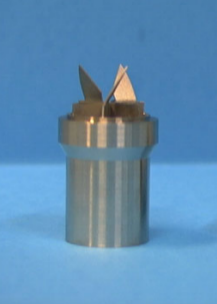
\includegraphics[height=4cm]{img/DEBORA-Promoteur/prom_pic.png}
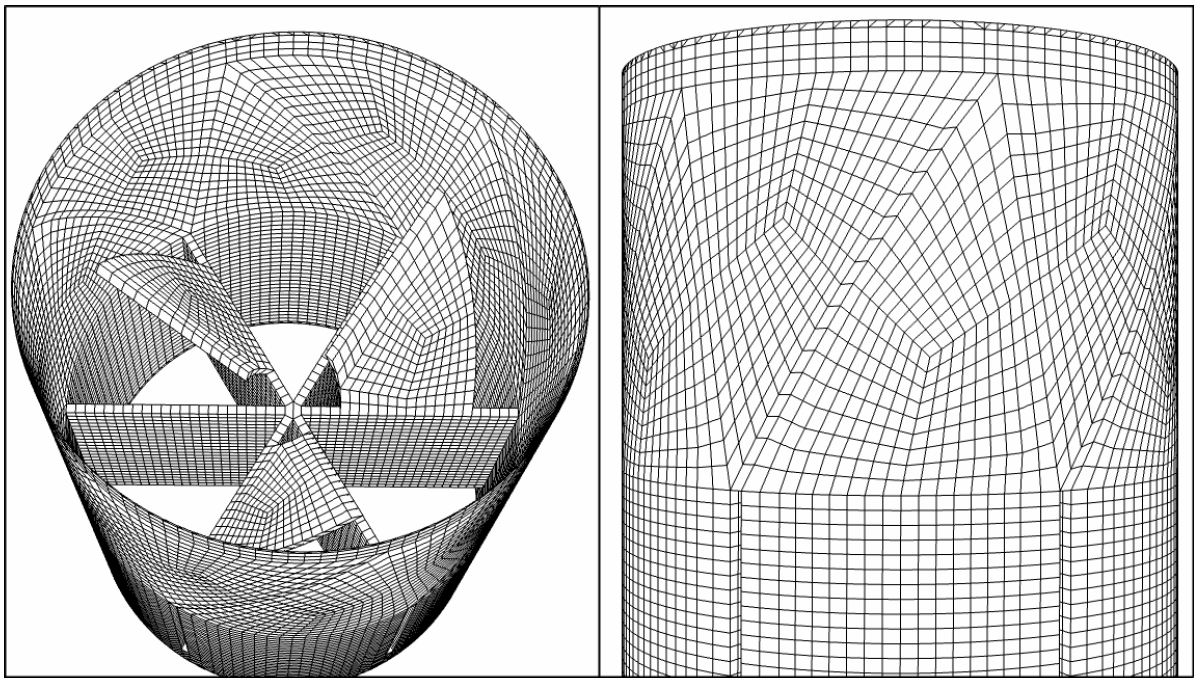
\includegraphics[height=4cm]{img/DEBORA-Promoteur/medium_mesh.PNG}
\caption{Picture of the mixing device (left) and its fine meshing (right).}
\label{fig:promoteur}
\end{figure}
%

Two series of measurements were conducted on this geometry : 

\begin{itemize}
\item Campaign 4800 : measurements of $\alpha$ using two optical probes, mixing device placed $0.455\text{m}\approx 23.5D_{h}$ upstream the end of the heating length
\item Campaign 5200 : measurements of $\alpha$ and $U_{G,z}$ using two optical probes, mixing device placed $0.192\text{m}\approx 10D_{h}$ upstream the end of the heating length
\end{itemize}

The goal of those tests was to observe the impact of the mixing device on the void fraction profile. The induced rotation is expected to gather the bubbles at the center of the tube and enhance condensation for highly subcooled cases. Those expectations are confirmed when looking at experimental $\alpha$ profiles on Figure \ref{fig:sim_prom}. The strong differences compared to simple tube profiles could explain the gain on the CHF value in PWR thanks to the mixing grids. Cases are named following the same nomenclature as presented in Section \ref{sec:deb_exp_campaign}.

\subsection{Analysis of the Experimental Measurements}



\begin{figure}[!h]
\centering
\subfloat[Void fraction]{
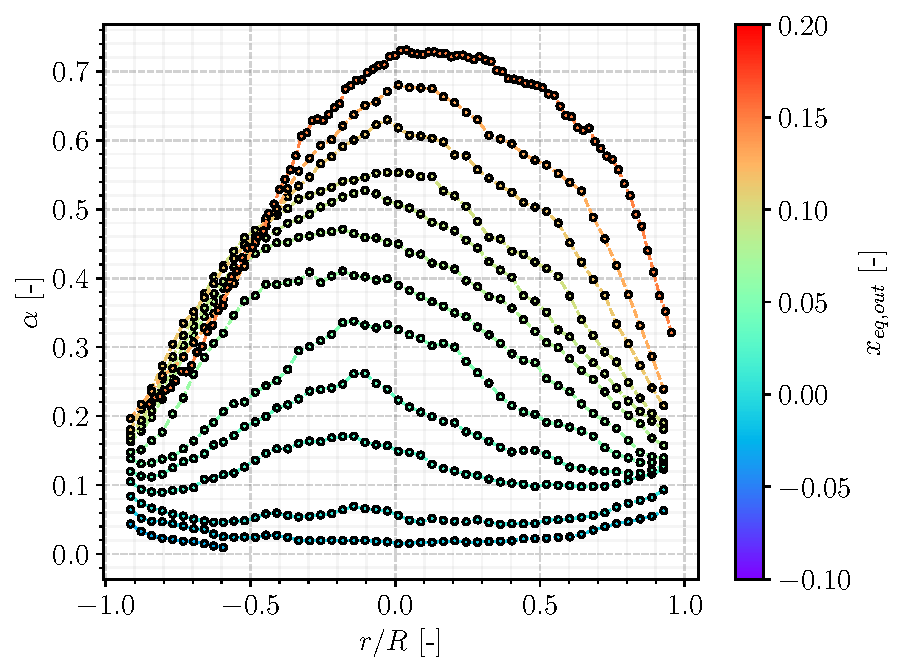
\includegraphics[width=0.5\linewidth]{img/DEBORA-Promoteur/48G3P26W23/48G3P26W23_alpha.pdf}
}
\subfloat[Interference frequency]{
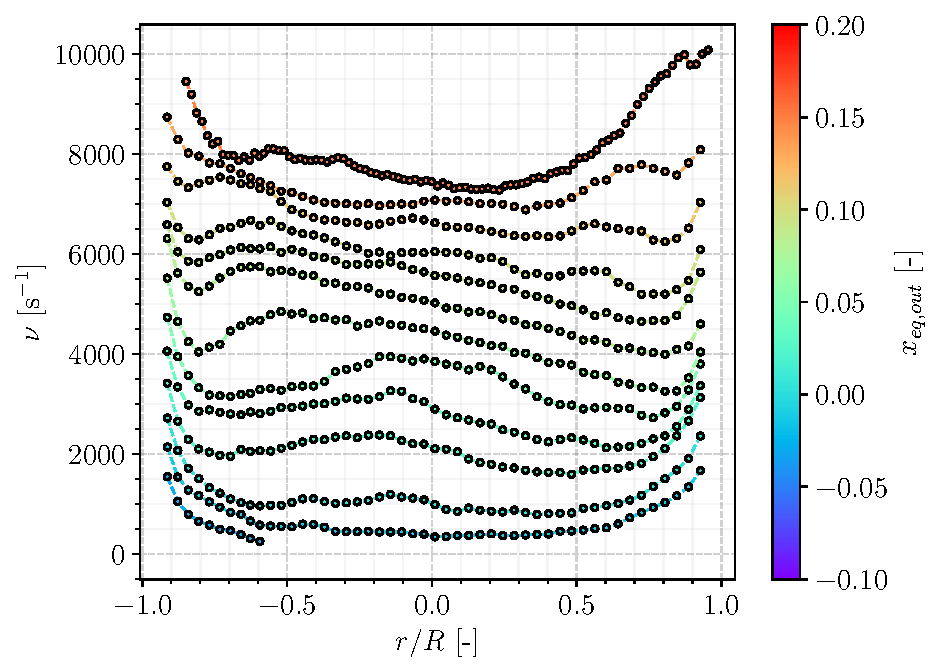
\includegraphics[width=0.5\linewidth]{img/DEBORA-Promoteur/48G3P26W23/48G3P26W23_nu.pdf}
}

\caption{Experimental results from the 48G3P26W23 series.}
\label{fig:exp_48G3P26W23}
\end{figure}


\begin{figure}[!h]
\centering
\subfloat[Void fraction]{
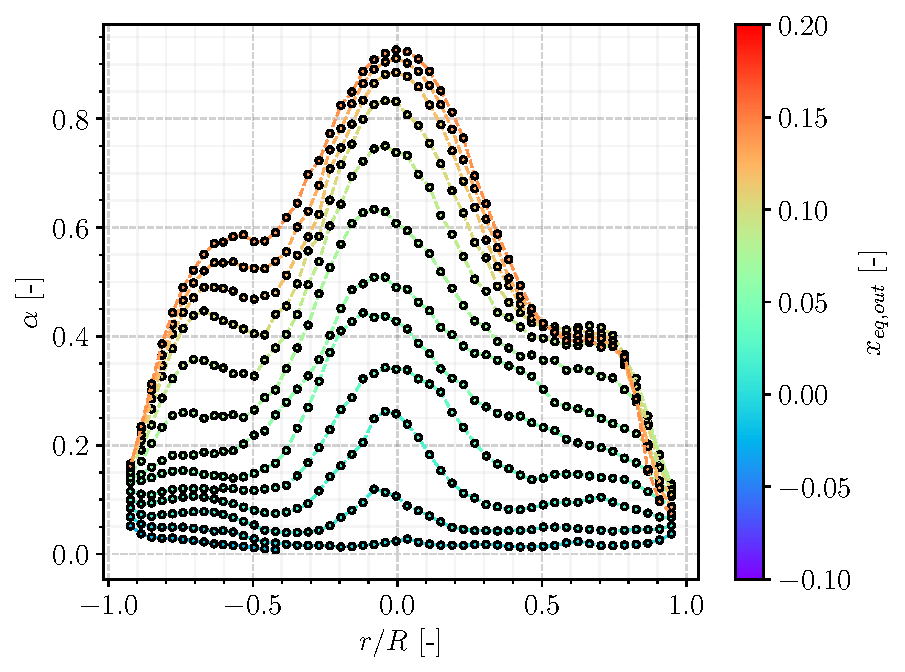
\includegraphics[width=0.5\linewidth]{img/DEBORA-Promoteur/52G3P26W23/52G3P26W23_alpha.pdf}
}
\subfloat[Interference frequency]{
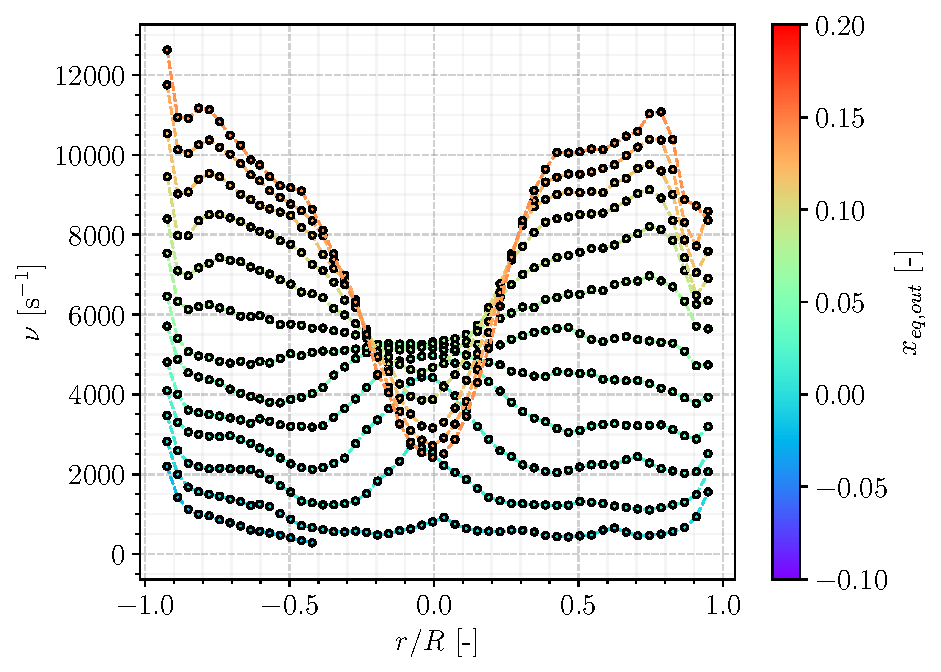
\includegraphics[width=0.5\linewidth]{img/DEBORA-Promoteur/52G3P26W23/52G3P26W23_nu.pdf}
}

\caption{Experimental results from the 52G3P26W23 series.}
\label{fig:exp_52G3P26W23}
\end{figure}


\begin{figure}[!h]
\centering
\subfloat[Void fraction]{
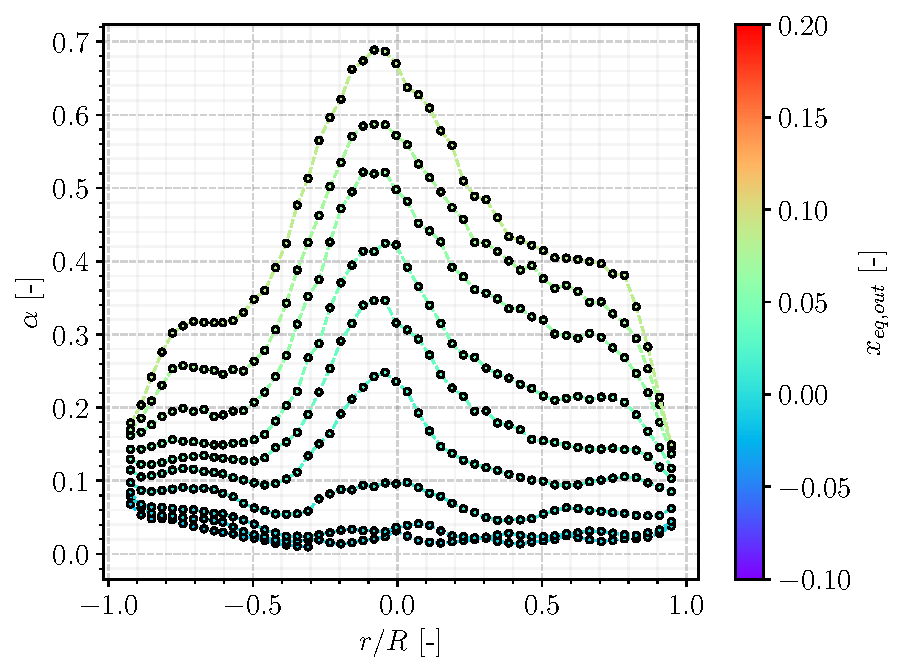
\includegraphics[width=0.5\linewidth]{img/DEBORA-Promoteur/52G3P26W27/52G3P26W27_alpha.pdf}
}
\subfloat[Interference frequency]{
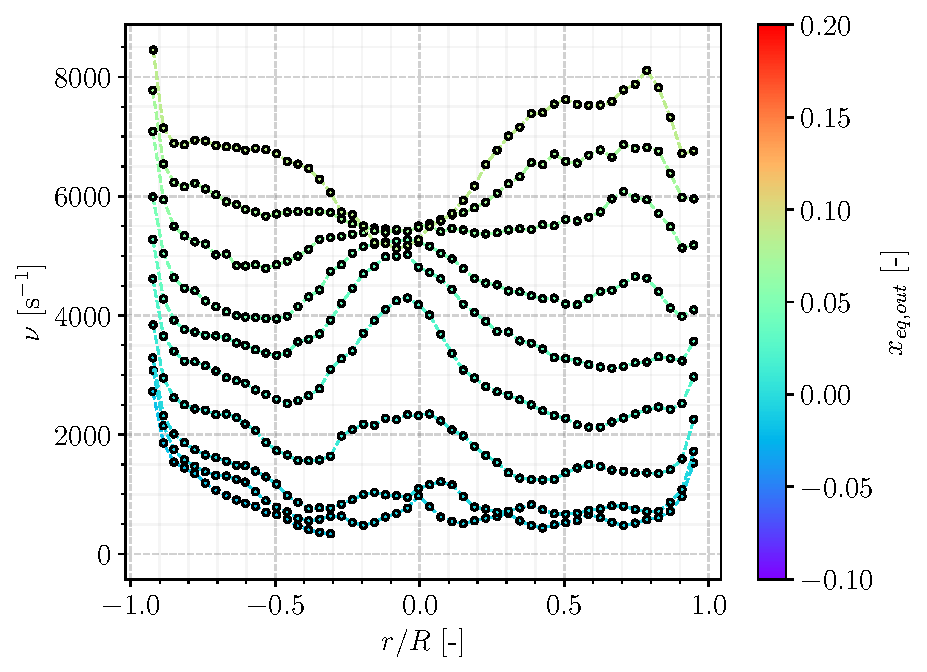
\includegraphics[width=0.5\linewidth]{img/DEBORA-Promoteur/52G3P26W27/52G3P26W27_nu.pdf}
}

\caption{Experimental results from the 52G3P26W27 series.}
\label{fig:exp_52G3P26W27}
\end{figure}




\begin{figure}[!h]
\centering
\subfloat[52G3P26W23 series]{
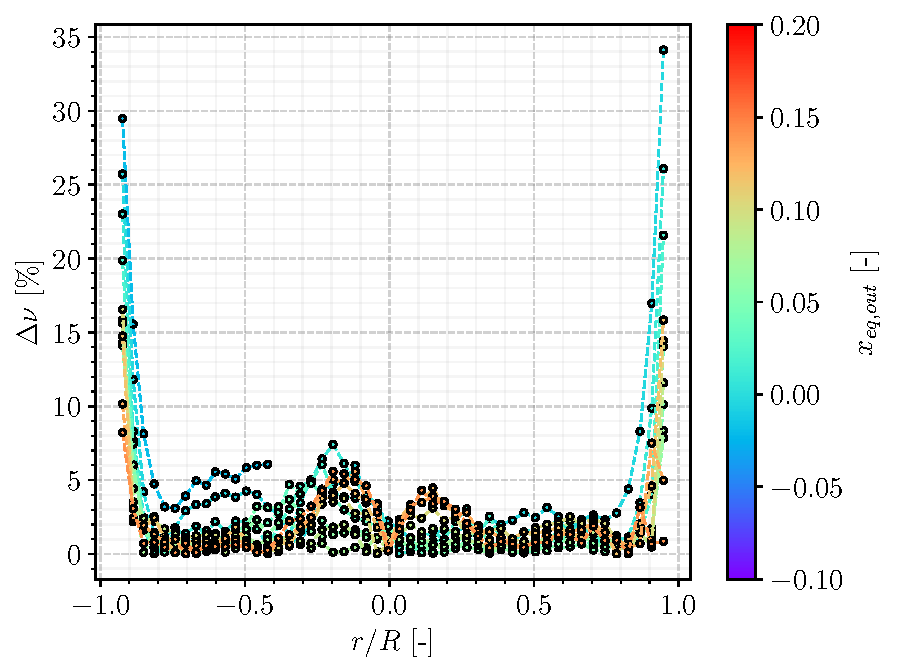
\includegraphics[width=0.5\linewidth]{img/DEBORA-Promoteur/52G3P26W23/52G3P26W23_deltanu.pdf}
}
\subfloat[52G3P26W27 series]{
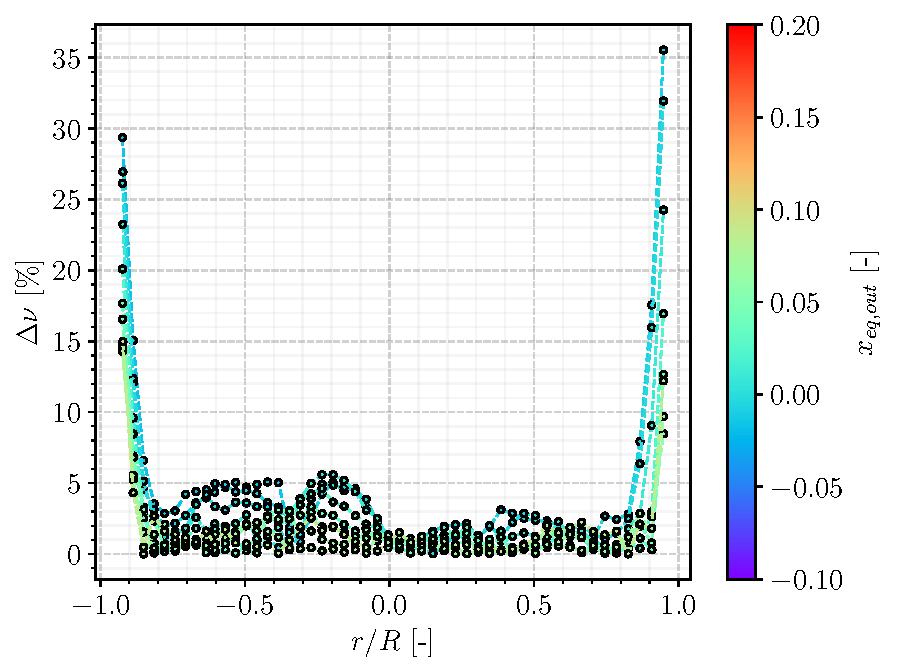
\includegraphics[width=0.5\linewidth]{img/DEBORA-Promoteur/52G3P26W27/52G3P26W27_deltanu.pdf}
}

\caption{Relative difference of interference frequency for the two probes.}
\label{fig:exp_C52_deltanu}
\end{figure}


\begin{figure}[!h]
\centering
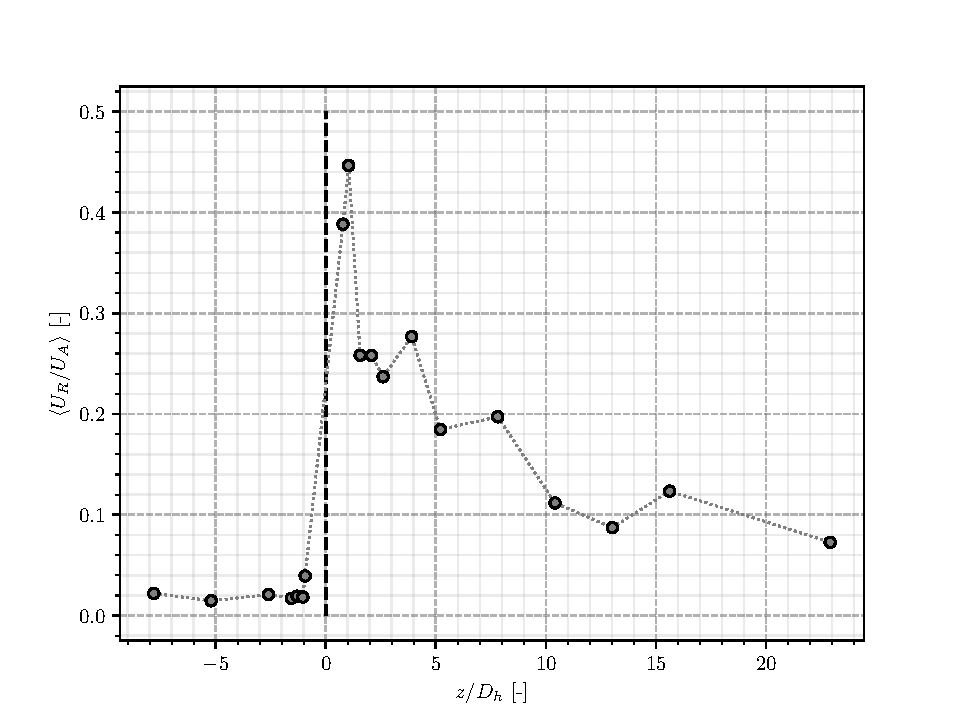
\includegraphics[width=0.5\linewidth]{img/AGATE/Urap_z.pdf}
\caption{Average relative importance of radial velocity to axial velocity in AGATE experiment}
\label{fig:exp_agate_Urap_z}
\end{figure}



\begin{figure}[!h]
\centering
\subfloat[52G3P26W23 series]{
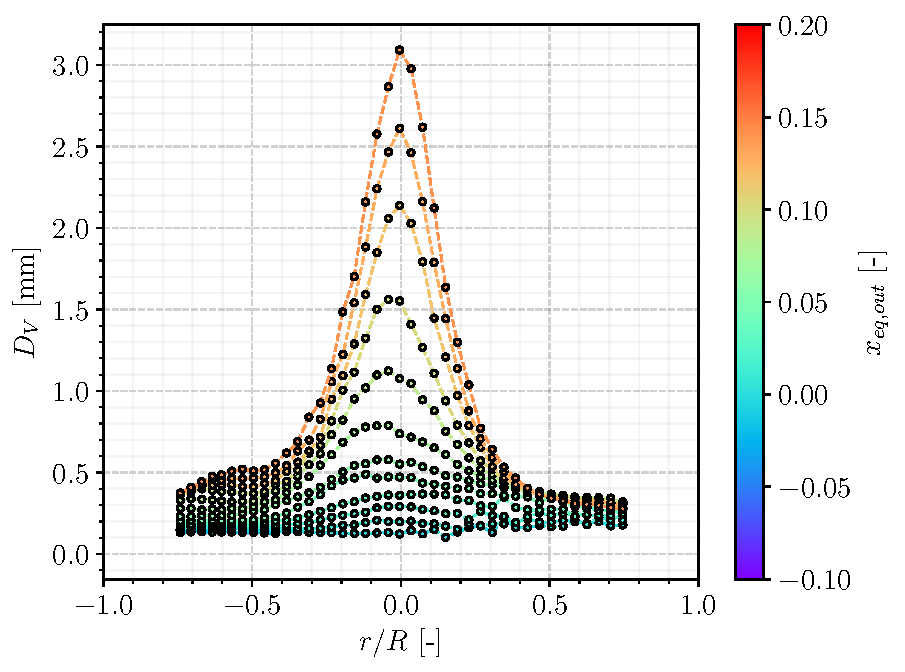
\includegraphics[width=0.5\linewidth]{img/DEBORA-Promoteur/52G3P26W23/52G3P26W23_dv.pdf}
}
\subfloat[52G3P26W27 series]{
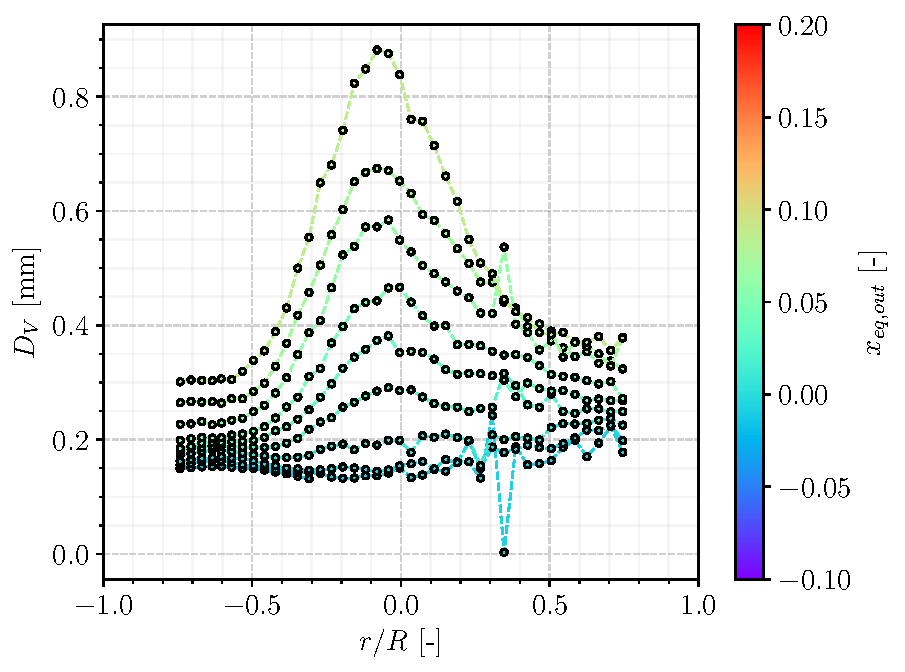
\includegraphics[width=0.5\linewidth]{img/DEBORA-Promoteur/52G3P26W27/52G3P26W27_dv.pdf}
}

\caption{Estimation of bubble diameter on C5200 measurements series.}
\label{fig:exp_C52_dvap}
\end{figure}




\subsection{NEPTUNE\_CFD simulations of DEBORA-Promoteur cases}

We simulated 3 cases for each position of the mixing device, covering different local thermodynamic quality near the vanes ($x_{eq,MV}$) :

\begin{itemize}
\item 48G3P26W23Te65 \& 52G3P26W23Te65 with $x_{eq,MV}\approx -1\%$ 
\item 48G3P26W23Te69 \& 52G3P26W23Te69 with $x_{eq,MV}\approx 4\%$ 
\item 48G3P26W23Te75 \& 52G3P26W23Te75 with $x_{eq,MV}\approx 12\%$ 
\end{itemize}

Computations are conducted using two meshes for Te69 cases : a large one (M1) with $444~703$ cells and a fine one (M2) with $3~487~627$ cells. Results for void fraction profiles are shown on Figure \ref{fig:sim_prom}.


%
\begin{figure}[!htb]
\centering
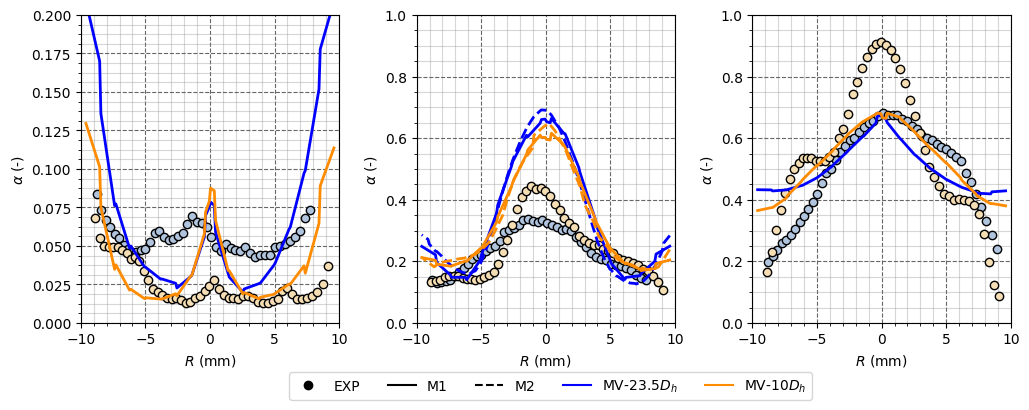
\includegraphics[scale=0.60]{img/DEBORA-Promoteur/alpha_prom.png}
\caption{NCFD (lines) vs. Exp. (circles) - $\alpha$ profiles for two MV positions (23.5$D_{h}$ in blue, $10D_{h}$ in orange) - $T_{in}=65\degree$C (left), $T_{in}=69\degree$C (middle), $T_{in}=75\degree$C (right) - Simulations using two meshes M1 (coarse) and M2 (fine) for $T_{in}=69\degree$C.}
\label{fig:sim_prom}
\end{figure}
%


Quantitatively speaking, it seems that NEPTUNE\_CFD reproduces the effect of vapor acculumation at the center thanks to the pressure gradient generated by the swirl induced by the mixing vanes. The radial position  of the core void fraction peak correctly matches the experimental one. 

However, measured void fraction profiles are not predicted correctly. A particularly strong overestimation of the core void fraction is observed as well as close to the wall. The CMFD results tend to rapidly reach a core void fraction around $60\%$ ($T_{in}=69\degree$C cases) and then flattens with increasing temperature ($T_{in}=75\degree$ cases). This contradicts experimental observation where the void fraction profile globally rises when inlet temperature increases, except at the wall where no peak is observed due to bubble removing effect by the liquid's rotation. Moreover, the $T_{in}=75\degree$ case with MV at $10D_{h}$ experimentally shows local $\alpha$ peaks at $R\approx \pm 6$mm which remain currently unexplained and not reproduced by the simulations. 

To investigate what could be a potential origin for the core void fraction peak overestimation, we present in Section \ref{sec:agate} single-phase flow simulations in the MV geometry.


\section{Liquid water flow in a tube with mixing vanes : AGATE-PROMOTEUR experiment}
\label{sec:agate}

In this penultimate section, we briefly investigate single-phase flow within the same geometry as Section \ref{sec:deb_prom}.

\subsection{Description of the experiment}

In 2003, using the same experimental geometry as DEBORA-Promoteur cases (Section \ref{sec:deb_prom}), Laser Doppler Velocimetry (LDV) measurements of velocity and turbulent fluctutations for an adiabatic single-phase flow of water were conducted. The outlet pressure was around $P=2$ bar with an inlet mass flux $G\approx 3000~\debm$. Measurements were conducted on $6$ different diameters and repeated at various axial positions upstream and downstream the mixing vanes.

A first look at experimental measurements (Figure \ref{fig:agate1}) shows that the vanes geometry induces significantly non-symmetric velocity profile. Moreover, we observe high turbulent fluctuations which maximum is located at the same radial position as the maximum radial velocity gradient.

\subsection{NEPTUNE\_CFD simulations of AGATE-Promoteur case}

On Figure \ref{fig:agate1}, we present some of the results obtained with NEPTUNE\_CFD using the $R_{ij}-\varepsilon~SSG$ turbulence model on the M2 mesh, along with a smooth wall law and a rough wall law (roughness $\epsilon=0.01$mm). The turbulent fluctuations Root Mean Square (RMS) correspond, for instance, to $\sqrt{<u^{'^{2}}_{x}>}$ for the $x$ direction where $u'_{i}$ represents the fluctuating part of the velocity along compononent $i$ and $<.>$ the time-averaging operator. Subscripts $R$ and $A$ stand for radial and axial values ; $U_{0}$ is the average inlet velocity.


%
\begin{figure}[!htb]
\centering
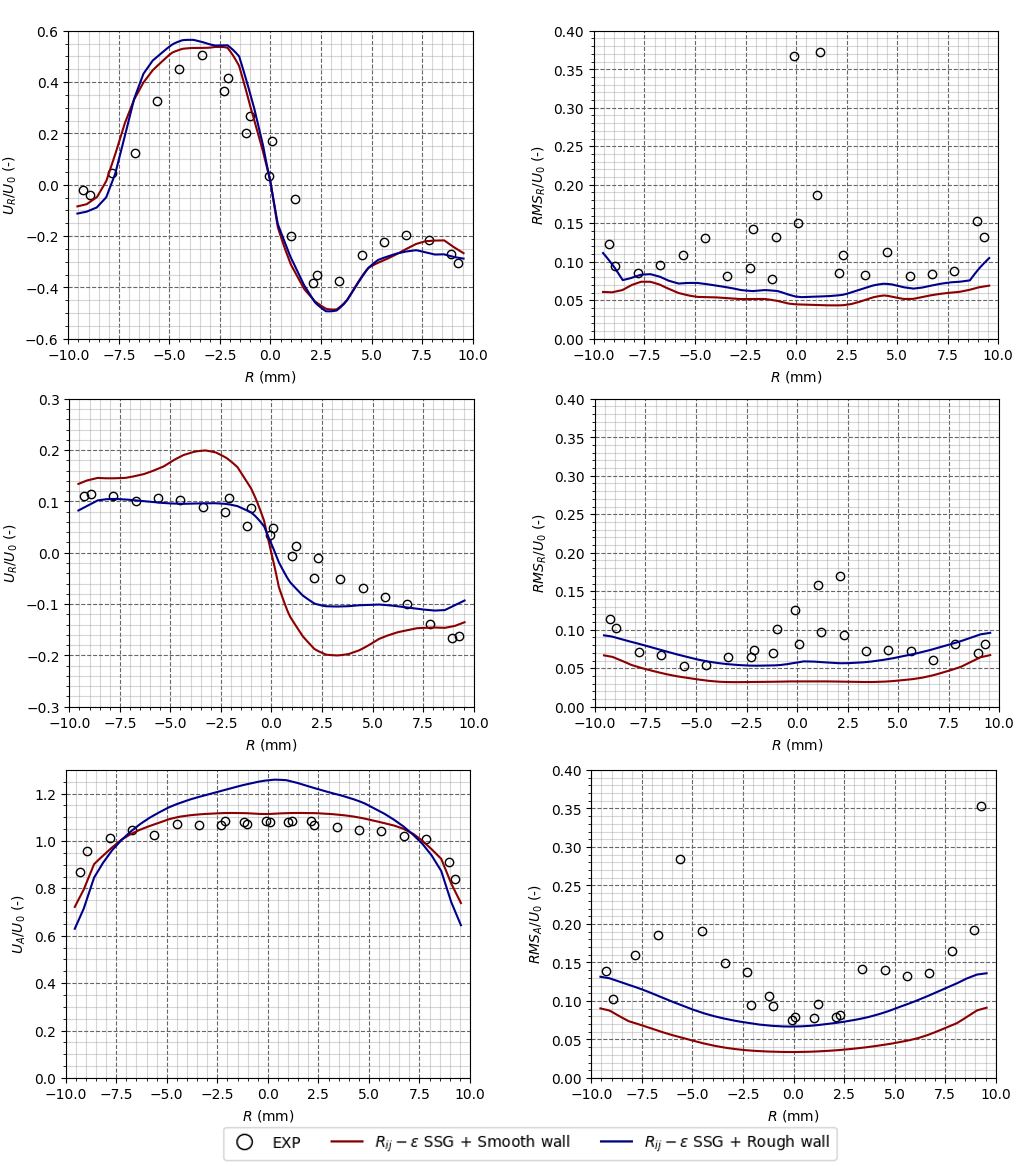
\includegraphics[scale=0.3]{img/AGATE/test.png}
\caption{NCFD vs. Exp. - Top \& Middle : Radial velocity and turbulent RMS ($z=30$mm \& $z=440$mm) -  Bottom : Axial velocity and turbulent RMS ($z=440$mm).}
\label{fig:agate1}
\end{figure}

Non-symmetric radial velocity profiles close to the MV are quite well reproduced by the simulations. However, far downstream the MV, it appears that the fluid's rotation is overestimated by the model with a smooth wall approach, while applying a roughness helps to reduce the magnitude of the swirl. Moreover, the radial turbulent fluctuations are better estimated by the rough wall approach at $z=440$~mm.

On the other hand, it seems that the rough wall approach deteriorates the axial velocity profile compared to the experiment. As shown on the bottom part of Figure \ref{fig:agate1}, the smooth wall simulation returns a flat velocity profile closer to the experiment than the rough wall one which overestimates the core velocity peak.

Both simulations globally underestimate the turbulent fluctuations, which can have a significant influence over the observed discrepancies on velocity profiles since turbulence plays a key role to homogenize the fluid flow. 

Those results finally highlight the fact that simulation of such rotating flows may need a particular wall approach to better capture the induced swirl and its dissipation. Correct prediction of turbulent fluctuations would be of significant interest to ensure liquid velocity validation. Further investigations on boiling cases could possibly be improved by a roughness approach, which is the current correction used for two-phase wall laws (Subsection \ref{subsec:wall_func}). 